\documentclass[12pt]{beamer}
\usetheme[progressbar=frametitle]{metropolis}
\usepackage{appendixnumberbeamer}
\usepackage{tabularx}
\usepackage{booktabs}
\usepackage[scale=2]{ccicons}
\usepackage{pgfplots}
\usepackage{xspace}
\usepackage{bm}
\usepackage{adjustbox}
\usepackage{xcolor}
\usepackage{changepage}
\usepgfplotslibrary{dateplot}
\setbeamercovered{transparent=30,again covered={\opaqueness<1->{30}}}

\title{Optimal Database Design Problem}
\author{Defended by: Group 06 \texorpdfstring{\\Magnani, Marchi, Moncada, Iaia,}{}\texorpdfstring{\\Palmieri, Ondesca, Ombe}{}}
\date{9, January 2019}
\institute{Politecnico di Torino\\Optimization Methods and Algorithms}

\begin{document}
  \maketitle
  \section{Algorithm presentation}
  % ------------------------------------------------------------------------------------------------------------
  %													Algorithm presentation
  % ------------------------------------------------------------------------------------------------------------
  {
  \usebackgroundtemplate{
\includegraphics[width=\paperwidth]{res/Genetic}}
  \color{white}
  \begin{frame}[fragile]{Genetic Algorithm}
    \begin{center}
      {\fontsize{30}{40}\selectfont \textbf{Why?}}
    \end{center}
  \end{frame}
  }

  \begin{frame}[fragile]{Main Features}
    \begin{columns}
      \begin{column}{0.5\textwidth}
        Key points of our implementation:
        \begin{itemize}
          \item<1> Scalability and adaptability
          \item<2> Multistart and restart
          \item<3> Multithreading
          \item<4> Large Solution Space exploration
        \end{itemize}
      \end{column}
      \begin{column}{0.5\textwidth}
          \only<1>{
            
\includegraphics[scale=0.2]{res/Scalability}
          }
          \only<2>{
            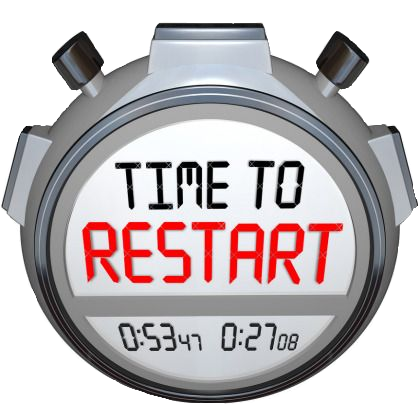
\includegraphics[scale=0.18]{res/Restart}
          }
          \only<3>{
            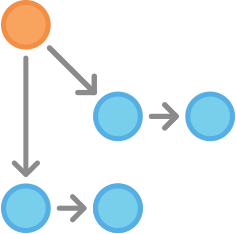
\includegraphics[scale=0.6]{res/Multithreading}
          }
          \only<4>{
            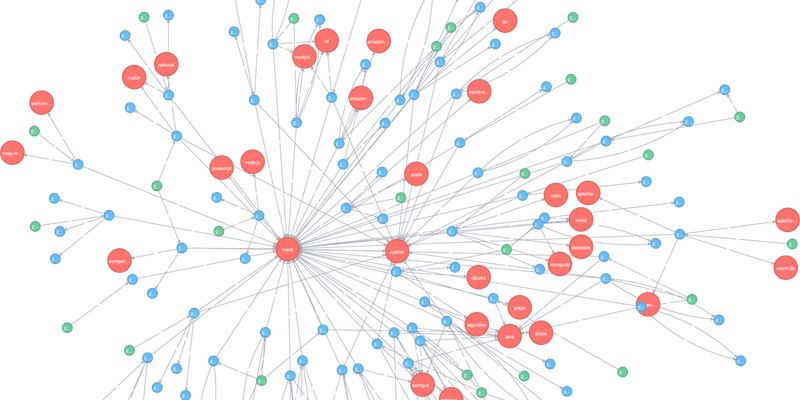
\includegraphics[scale=0.8]{res/SolutionSpace}
          }
      \end{column}
    \end{columns}
  \end{frame}

  \begin{frame}[fragile]{Solution Set Selection procedures}
    \begin{columns}
      \begin{column}{0.5\textwidth}
        Solution Set Selection procedures implemented:
        \begin{itemize}
          \item<1> Roulette
          \item<2> Tournament
          \item<3> Random
        \end{itemize}
      \end{column}
      \begin{column}{0.5\textwidth}
          \only<1>{
            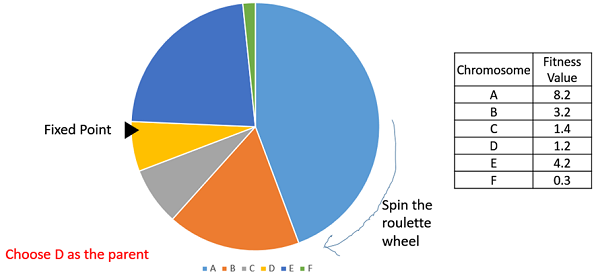
\includegraphics[scale=1.0]{res/Roulette}
          }
          \only<2>{
            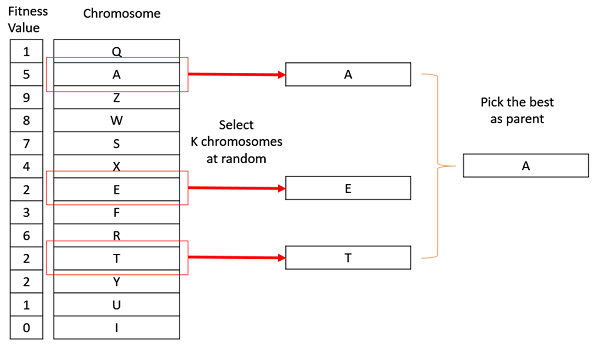
\includegraphics[scale=1.0]{res/Tournament}
          }
          \only<3>{
            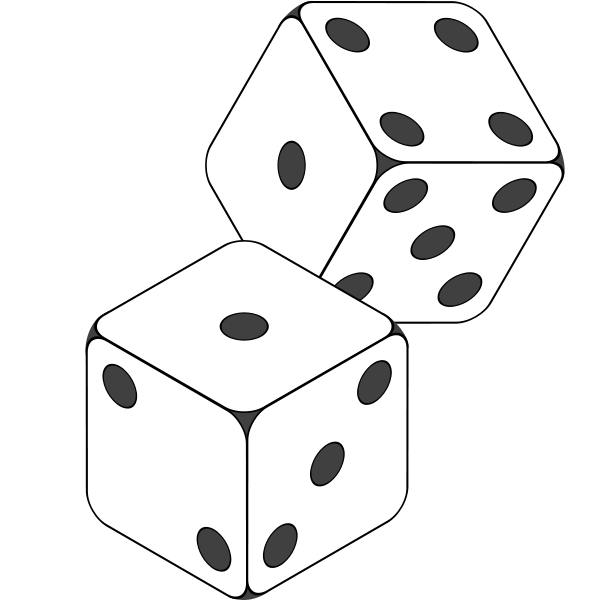
\includegraphics[scale=0.15]{res/Random}
          }
      \end{column}
    \end{columns}
  \end{frame}

  \begin{frame}[fragile]{Children generation methods}
    Children generation methods implemented:
    \begin{itemize}
      \item Mutation
      \begin{itemize}
        \item 2-bit instead of 1
        \item 70\% chance to be chosen
      \end{itemize}
      \item Inversion
      \begin{itemize}
        \item traditional approach adapted to the instance dimension
        \item 15\% chance to be chosen
      \end{itemize}
      \item Crossover
       \begin{itemize}
        \item traditional approach
        \item 15\% change to be chosen
      \end{itemize}
    \end{itemize}
  \end{frame}

  \begin{frame}[fragile]{Algorithm steps}
    \begin{adjustwidth}{-2em}{-2em}
      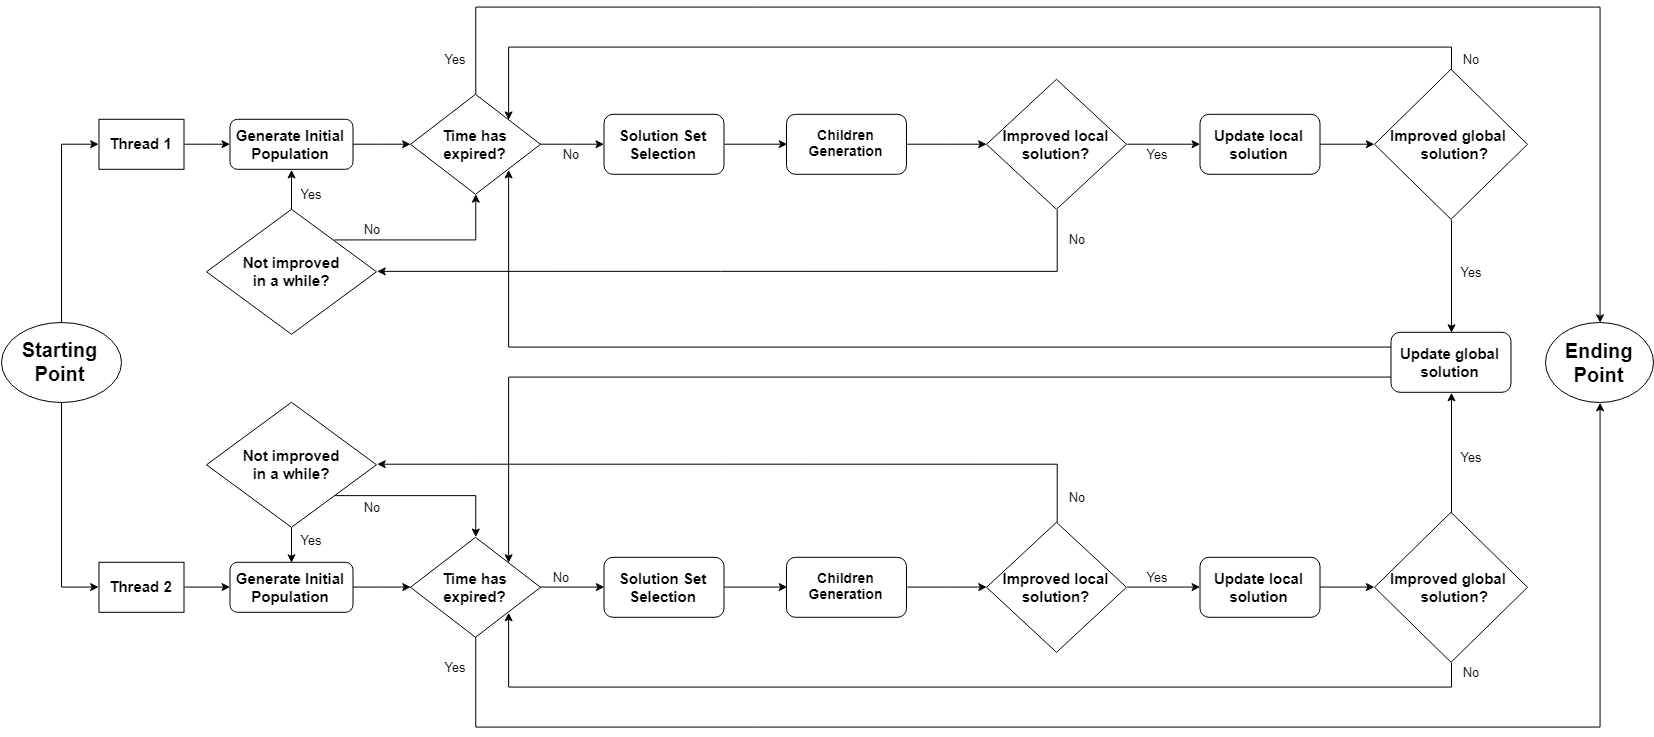
\includegraphics[scale=0.21]{res/Algorithm}
    \end{adjustwidth}
  \end{frame}

  \section{Results analysis}
  % ------------------------------------------------------------------------------------------------------------
  %													Results
  % ------------------------------------------------------------------------------------------------------------
  \begin{frame}[fragile]{Result Analysis}
    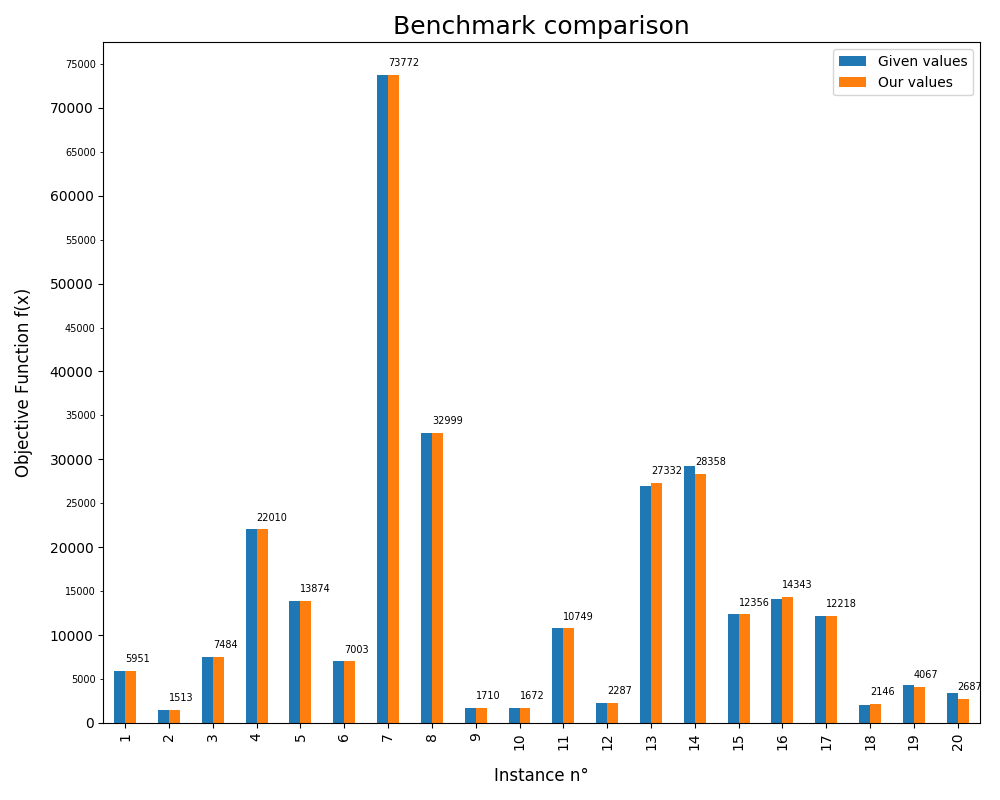
\includegraphics[scale=0.4]{res/benchmarkComparison}
  \end{frame}

  % ------------------------------------------------------------------------------------------------------------
  %													End
  % ------------------------------------------------------------------------------------------------------------
  \begin{frame}[standout]
  	THE END
  \end{frame}

\end{document}